% $Id: template.tex 11 2007-04-03 22:25:53Z jpeltier $

\documentclass{vgtc}                          % final (conference style)
%\documentclass[review]{vgtc}                 % review
%\documentclass[widereview]{vgtc}             % wide-spaced review
%\documentclass[preprint]{vgtc}               % preprint
%\documentclass[electronic]{vgtc}             % electronic version

%% Uncomment one of the lines above depending on where your paper is
%% in the conference process. ``review'' and ``widereview'' are for review
%% submission, ``preprint'' is for pre-publication, and the final version
%% doesn't use a specific qualifier. Further, ``electronic'' includes
%% hyperreferences for more convenient online viewing.

%% Please use one of the ``review'' options in combination with the
%% assigned online id (see below) ONLY if your paper uses a double blind
%% review process. Some conferences, like IEEE Vis and InfoVis, have NOT
%% in the past.

%% Figures should be in CMYK or Grey scale format, otherwise, colour 
%% shifting may occur during the printing process.

%% These few lines make a distinction between latex and pdflatex calls and they
%% bring in essential packages for graphics and font handling.
%% Note that due to the \DeclareGraphicsExtensions{} call it is no longer necessary
%% to provide the the path and extension of a graphics file:
%% \includegraphics{diamondrule} is completely sufficient.
%%
\ifpdf%                                % if we use pdflatex
  \pdfoutput=1\relax                   % create PDFs from pdfLaTeX
  \pdfcompresslevel=9                  % PDF Compression
  \pdfoptionpdfminorversion=7          % create PDF 1.7
  \ExecuteOptions{pdftex}
  \usepackage{graphicx}                % allow us to embed graphics files
  \DeclareGraphicsExtensions{.pdf,.png,.jpg,.jpeg} % for pdflatex we expect .pdf, .png, or .jpg files
\else%                                 % else we use pure latex
  \ExecuteOptions{dvips}
  \usepackage{graphicx}                % allow us to embed graphics files
  \DeclareGraphicsExtensions{.eps}     % for pure latex we expect eps files
\fi%

%% it is recomended to use ``\autoref{sec:bla}'' instead of ``Fig.~\ref{sec:bla}''
\graphicspath{{figures/}{pictures/}{images/}{./}} % where to search for the images

\usepackage{microtype}                 % use micro-typography (slightly more compact, better to read)
\PassOptionsToPackage{warn}{textcomp}  % to address font issues with \textrightarrow
\usepackage{textcomp}                  % use better special symbols
\usepackage{mathptmx}                  % use matching math font
\usepackage{times}                     % we use Times as the main font
\renewcommand*\ttdefault{txtt}         % a nicer typewriter font
\usepackage{cite}                      % needed to automatically sort the references
\usepackage{tabu}                      % only used for the table example
\usepackage{booktabs}                  % only used for the table example
%% We encourage the use of mathptmx for consistent usage of times font
%% throughout the proceedings. However, if you encounter conflicts
%% with other math-related packages, you may want to disable it.

%% If you are submitting a paper to a conference for review with a double
%% blind reviewing process, please replace the value ``0'' below with your
%% OnlineID. Otherwise, you may safely leave it at ``0''.
\onlineid{0}

%% declare the category of your paper, only shown in review mode
\vgtccategory{Research}

%% allow for this line if you want the electronic option to work properly
\vgtcinsertpkg

%% In preprint mode you may define your own headline. If not, the default IEEE copyright message will appear in preprint mode.
%\preprinttext{To appear in an IEEE VGTC sponsored conference.}

%% This adds a link to the version of the paper on IEEEXplore
%% Uncomment this line when you produce a preprint version of the article 
%% after the article receives a DOI for the paper from IEEE
%\ieeedoi{xx.xxxx/TVCG.201x.xxxxxxx}

\usepackage[nameinlink]{cleveref}
\usepackage[nolist,nohyperlinks]{acronym}
\acrodef{VIS}{Data Visualization and Visual Analytics}
\acrodef{SCRC}{The Scottish COVID-19 Response Consortium}

%% Paper title.

\title{EnsembleVis: A Retrospective and Early History}

%% This is how authors are specified in the conference style

%% Author and Affiliation (single author).
%%\author{Roy G. Biv\thanks{e-mail: roy.g.biv@aol.com}}
%%\affiliation{\scriptsize Allied Widgets Research}

%% Author and Affiliation (multiple authors with single affiliations).
%%\author{Roy G. Biv\thanks{e-mail: roy.g.biv@aol.com} %
%%\and Ed Grimley\thanks{e-mail:ed.grimley@aol.com} %
%%\and Martha Stewart\thanks{e-mail:martha.stewart@marthastewart.com}}
%%\affiliation{\scriptsize Martha Stewart Enterprises \\ Microsoft Research}

%% Author and Affiliation (multiple authors with multiple affiliations)
\author{Qiru Wang\thanks{e-mail: qiru.wang1@nottingham.ac.uk}\\ %
        \scriptsize University of Nottingham %
\and Robert S. Laramee\thanks{e-mail: robert.laramee@nottingham.ac.uk}\\ %
     \scriptsize University of Nottingham}

%% A teaser figure can be included as follows
\teaser{
  \centering
  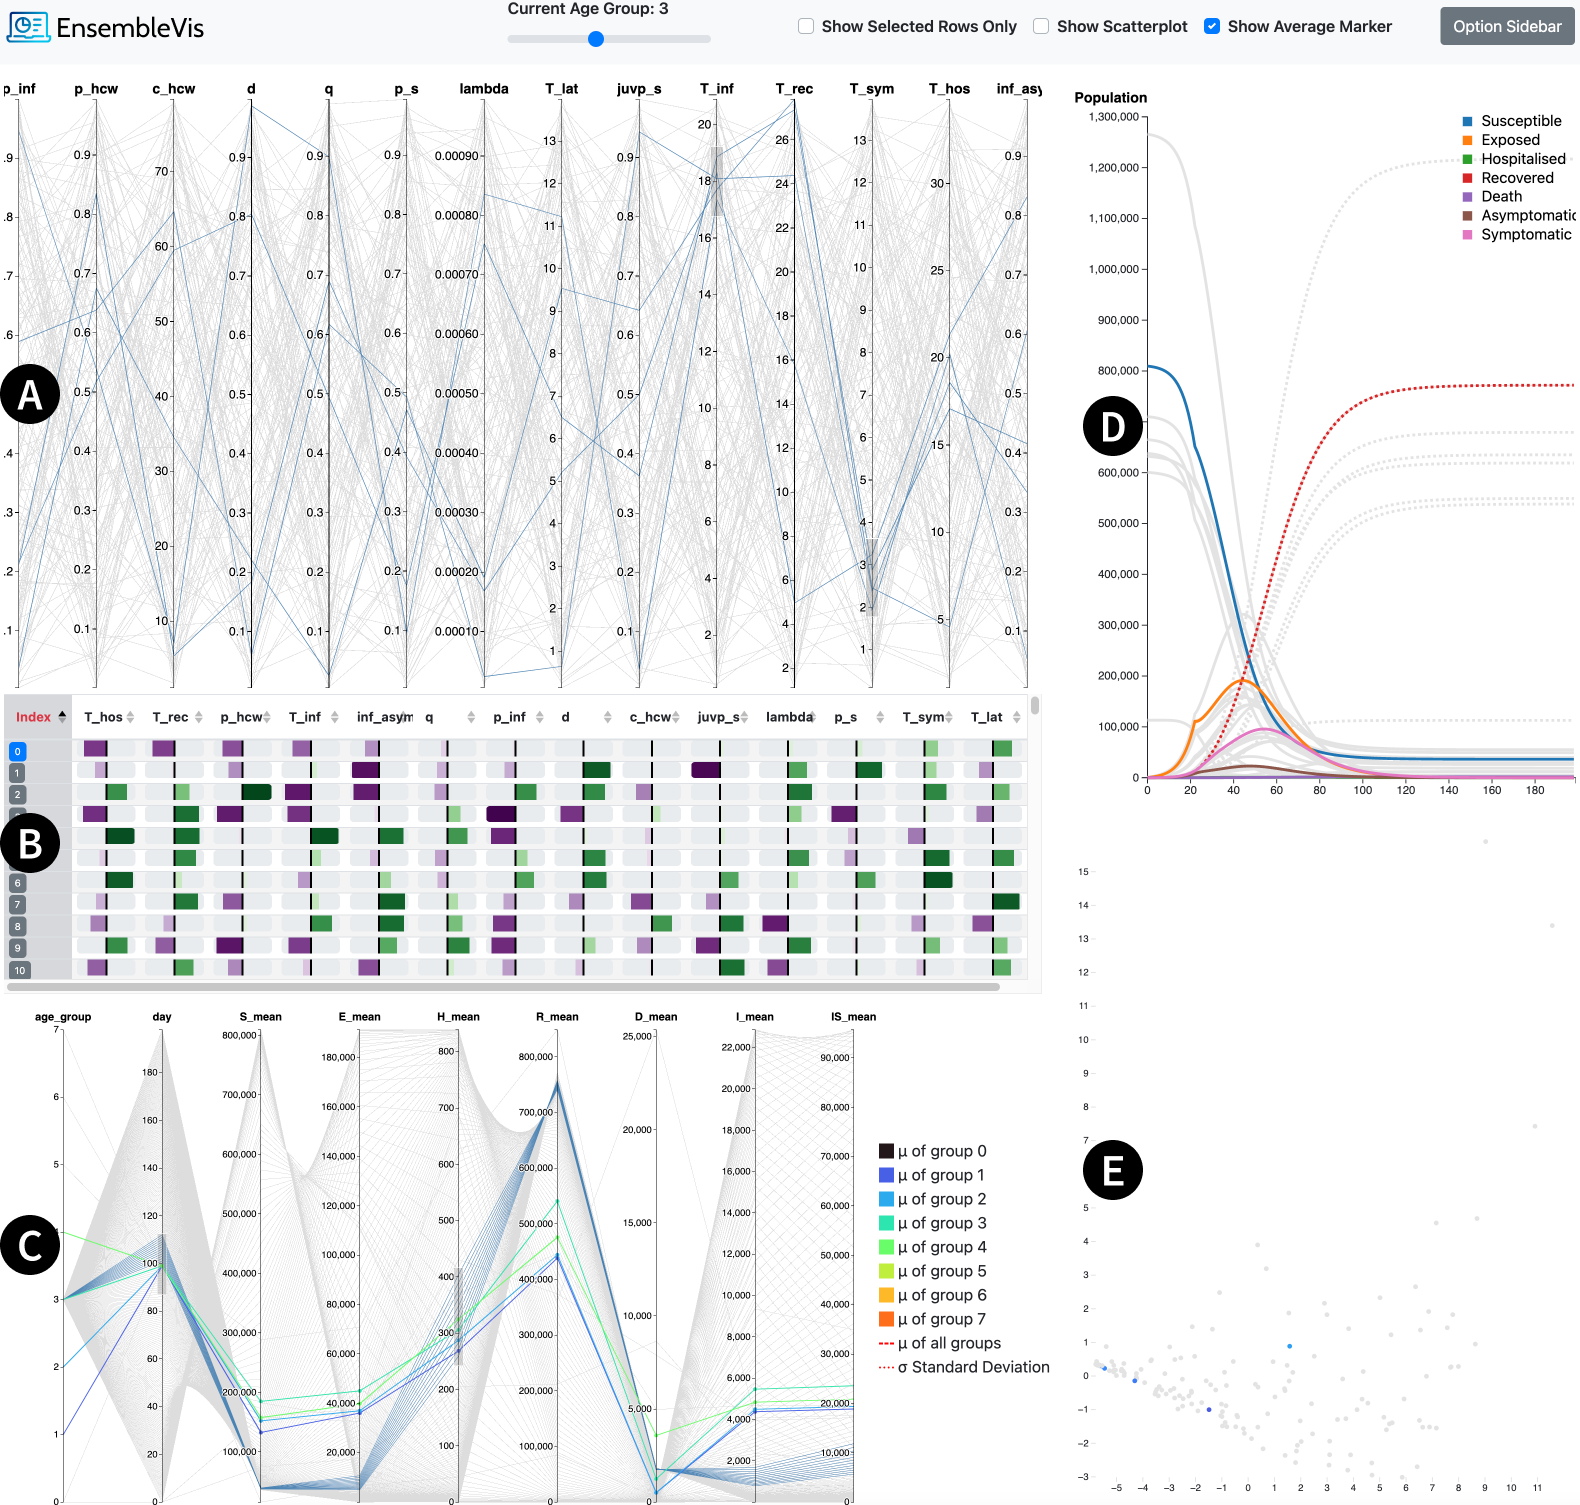
\includegraphics[width=\linewidth]{overview.png}
  \caption{An overview of EnsembleVis, an interactive dashboard designed for visualizing the input parameters and outcomes of an ABC-smc inference model used for analyzing COVID-19 data collected during the first wave of the outbreak in Scotland \cite{2020Covid19}. Its main purpose is to facilitate a better understanding of the complex dynamics of the pandemic by presenting the relationships between different sets of input parameters and the resulting outcomes in a clear and intuitive manner. A detailed description of the dashboard can be found in \Cref{sec:EnsembleVis}.
  }
  \label{fig:teaser}
}

%% Abstract section.
\abstract{
} % end of abstract

%% ACM Computing Classification System (CCS). 
%% See <http://www.acm.org/about/class> for details.
%% We recommend the 2012 system <http://www.acm.org/about/class/class/2012>
%% For the 2012 system use the ``\CCScatTwelve'' which command takes four arguments.
%% The 1998 system <http://www.acm.org/about/class/class/2012> is still possible
%% For the 1998 system use the ``\CCScat'' which command takes four arguments.
%% In both cases the last two arguments (1998) or last three (2012) can be empty.

\CCScatlist{
  \CCScatTwelve{Visual Analytics}{Information Visualization}{Emergency Response}{Visual Design}
}

%\CCScatlist{
  %\CCScat{H.5.2}{User Interfaces}{User Interfaces}{Graphical user interfaces (GUI)}{};
  %\CCScat{H.5.m}{Information Interfaces and Presentation}{Miscellaneous}{}{}
%}

%% Copyright space is enabled by default as required by guidelines.
%% It is disabled by the 'review' option or via the following command:
% \nocopyrightspace

%%%%%%%%%%%%%%%%%%%%%%%%%%%%%%%%%%%%%%%%%%%%%%%%%%%%%%%%%%%%%%%%
%%%%%%%%%%%%%%%%%%%%%% START OF THE PAPER %%%%%%%%%%%%%%%%%%%%%%
%%%%%%%%%%%%%%%%%%%%%%%%%%%%%%%%%%%%%%%%%%%%%%%%%%%%%%%%%%%%%%%%%

\begin{document}

%% The ``\maketitle'' command must be the first command after the
%% ``\begin{document}'' command. It prepares and prints the title block.

%% the only exception to this rule is the \firstsection command
% \firstsection{Introduction}

\maketitle

\section{Introduction and Motivation}
\label{sec:intro}

The Scottish COVID-19 Response Consortium (SCRC) \cite{2020University}, in collaboration with the Royal Society's call to action in March 2020, has taken a proactive approach to address the need for enhanced epidemiological models of COVID-19 transmission.
This joint volunteer effort, known as Rapid Assistance in Modeling the Pandemic (RAMP) \cite{2020Rapid}, aims to foster a deeper understanding of the consequences associated with various exit strategies from lockdown measures.
Moreover, this consortium attracted the involvement of distinguished scientists and experts from diverse organizations both within the United Kingdom and abroad, thus augmenting the collective knowledge base and ensuring comprehensive expertise in specialized domains.

RAMPVis \cite{2020Visualization} is a group of researchers specialized in Data Visualization and Visual Analytics (abbreviated as VIS).
This group voluntarily came forward to contribute its specialized skills and knowledge in order to provide valuable support to the SCRC modelers.
The term \textit{modelers} used here refers to the SCRC researchers who were actively engaged in the development of epidemiological models in the SCRC.
% revision 
This target user group predominantly includes experts in domains such as mathematics, statistics, and epidemiology.

Serving as the volunteer team responsible for providing visualization support to one of the epidemiological models developed by the SCRC modelers \cite{chen2022RAMPVIS}, our main objective is to provide VIS researchers and practitioners with valuable insights gained from our research and development (R\&D) activities conducted during the COVID-19 pandemic.
In an effort to predict the potential impact of diverse interventions, modelers have actively utilized COVID-19 data, employing a method known as Uncertainty Quantification (UQ).
This process seeks to measure uncertainties through the application of mathematical models and simulations.
However, modelers are faced with significant challenges, including the aspects of expert elicitation and effective communication.
In other words, there is a need for software engineering effort coupled with visualization to provide support for the validation and verification tests, and to create efficient workflows between modelers and researchers from other disciplines \cite{ackland2022Royal}.

\begin{figure}[tb!]
    \centering
    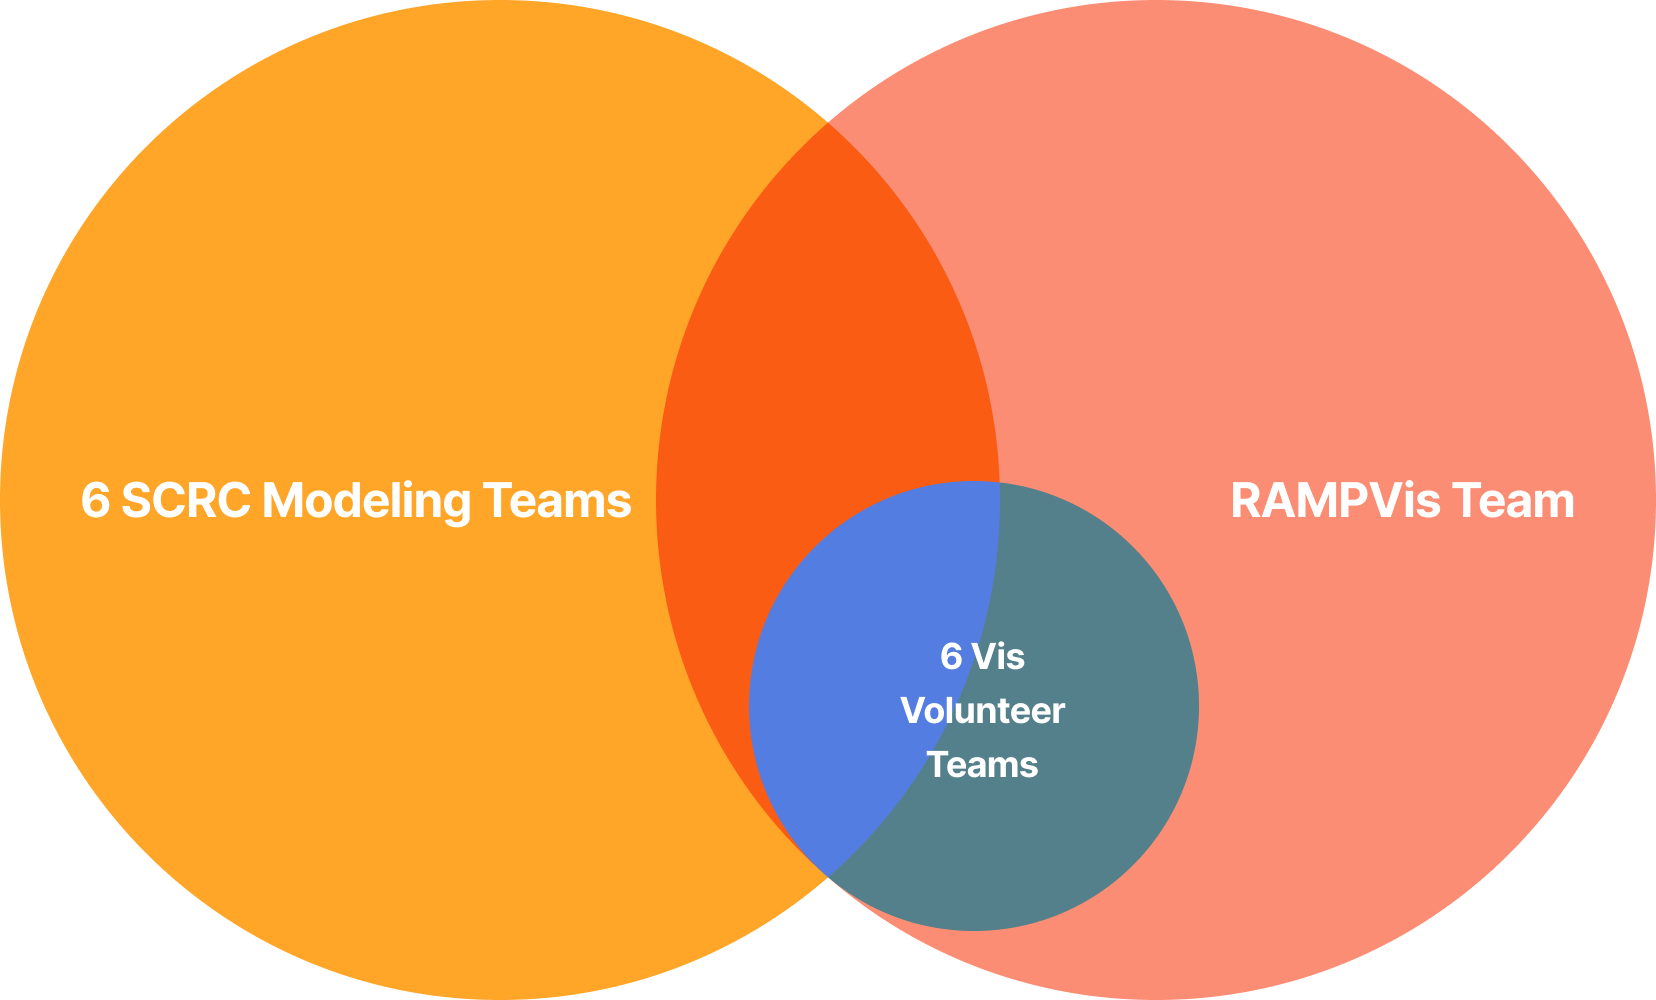
\includegraphics[width=0.65\linewidth]{venn.png}
    \caption{The organization of researchers from the SCRC and RAMPVis. The SCRC modeling team is responsible for developing the epidemiological models leveraging different modeling techniques. The RAMPVis team provides visualization support to the SCRC modeling team, by establishing four VIS volunteer teams who work on the actual development under the guidance of the RAMPVis team.
    }
    \label{fig:venn}

\end{figure}

In addressing these hurdles, \ac{VIS} emerge as a potent tool, offering the capacity to significantly enhance and streamline their collaborative workflows \cite{swallow2022Challenges}.
While our work may not have showcased the state-of-the-art VIS techniques, it effectively delivered rapid and practical VIS support to the modelers during an exceptional and demanding time.

Our contribution is an early history of our volunteer response from a software engineering and visualization perspective.
We present the earliest stages of the visualization dashboard, EnsembleDashVis, developed during the pandemic, aiming to assist the modelers in interpreting an \ac{ABC-SMC} inference model that they have developed using COVID-19 data collected during the first wave of the outbreak in Scotland \cite{scrc2020Covid19}. 
Much of this effort and the reasoning behind this volunteer work was never documented.

% revision
\noindent
\textbf{Unconventional Software Development:}  
The visualization software we developed in this project was developed under unconventional and unprecedented circumstances.
Some of the unusual properties of this software project were the amount of uncertainty as the project started.
The following aspects were unknown at the project start:
\begin{itemize}[itemsep=0pt,topsep=0pt]
    \item An unknown a priori requirements specification: We did not know what the user requirements and expectations were.
    \item An unknown project team: The members of the project team were unknown.
    We only knew the leader of the visualization team, Prof Min Chen. 
    In addition, the project team was dynamic with new members joining throughout.
    \item Unknown data characteristics: We did not know what the simulation data was at the start of the project.
    \item An unfamiliar work environment: The collective work environment landscape shifted to a work-at-home model which was new to the team at the time.
\end{itemize}
While arguably, these characteristics could describe other software engineering projects, we believe that the uncertainty in this particular case was unusually high.
All aspects of this project had the feel of laying down the tracks as the train was running.

\section{Background and Related Work}

\ac{VIS} has been extensively utilized in critical applications and healthcare, including during the COVID-19 pandemic.
Data visualization has played a prominent role in disseminating COVID-19 information through various media channels.
This surge in \ac{VIS} adoption has facilitated a better understanding of the pandemic's impact, aided in identifying trends and patterns, and empowered decision-makers with actionable insights derived from complex datasets.

Our work is included in multiple publications \cite{chen2022RAMPVIS,dykes2022Visualizationb,khan2022Propagating,rydow2023RAMPVIS}, as the foundation for their implementations.
As we have already described the related work in \ac{VIS} in emergency response and healthcare behind our implementation (See related work section in Chen et al. \cite{chen2022RAMPVIS}), in this section, we will provide a concise exploration of the various applications of \ac{VIS} in these domains, which served as a catalyst for our own development efforts.

In contrast to the majority of previous studies that typically focus on preparing for future emergencies, our work was undertaken during the COVID-19 pandemic as a rapid response to an ongoing emergency.

\section{Data Description}
\label{sec:Data}

\begin{table}[tb!]
    \centering
    \caption{16 input parameters for the ABC-SMC inference model. As constant parameters such as $K$ and $rrd$ do not affect the simulation results, they are not rendered in our visual designs.}
    \label{tab:input_params}
    \resizebox{\columnwidth}{!}{%
        \begin{tabular}{|l|l|}
            \hline
            \textbf{Name} & \textbf{Description}                                                       \\
            \hline
            \hline
            T\_lat        & Mean latent period (days)                                                  \\
            \hline
            juvp\_s       & Probability of juvenile developing symptoms                                \\
            \hline
            T\_inf        & Mean asymptomatic period (days)                                            \\
            \hline
            T\_rec        & Mean time to recovery if symptomatic (days)                                \\
            \hline
            T\_sym        & Mean symptomatic period prior to hospitalization (days)                    \\
            \hline
            T\_hos        & Mean hospitalization stay (days)                                           \\
            \hline
            inf\_asym     & Reduction factor of infectiousness for asymptomatic infectious individuals \\
            \hline
            p\_inf        & Probability of Infection                                                   \\
            \hline
            p\_hcw        & Probability of Infection (Healthcare Worker)                               \\
            \hline
            c\_hcw        & Mean number of Healthcare Worker contacts per day                          \\
            \hline
            d             & Proportion of population observing social distancing                       \\
            \hline
            q             & Proportion of normal contact made by people self-isolating                 \\
            \hline
            p\_s          & Age-dependent probability of developing symptoms                           \\
            \hline
            rrd           & Risk of death if not hospitalized                                          \\
            \hline
            lambda        & Background transmission rate                                               \\
            \hline
            K             & Hospital bed capacity                                                      \\
            \hline
        \end{tabular}
    }
\end{table}

\begin{table}[tb!]
    \centering
    \caption{13 output parameters from the simulation performed by the ABC-SMC inference model.}
    \label{tab:output_param}
    \resizebox{\columnwidth}{!}{%
        \begin{tabular}{|l|p{9.25cm}|}
            \hline
            \textbf{Name} & \textbf{Description}
            \\
            \hline
            \hline

            iter          & The simulation number.
            \\
            \hline
            day           & The day number.
            \\
            \hline
            age\_group    & The age group of the population.
            \\
            \hline
            S             & Number of susceptible individuals (not infected).                                                           \\
            \hline
            E             & Number of infected individuals but not yet infectious (exposed).                                            \\
            \hline
            E\_t          & Number of exposed individuals and tested positive.                                                          \\
            \hline
            I\_p          & Number of infected and infectious symptomatic individuals but at pre-clinical stage (show yet no symptoms). \\
            \hline
            I\_t          & Number of tested positive individuals that are infectious.                                                  \\
            \hline
            I            & Number of infected and infectious asymptomatic individuals.                                    \\
            \hline
            I\_s         & Number of infected and infectious symptomatic individuals.                                     \\
            \hline
            H             & Number of infected individuals that are hospitalized.                                                       \\
            \hline
            R             & Number of infected individuals that have recovered from the infection.                                      \\
            \hline
            D             & Number of deceased individuals due to the disease.                                                          \\
            \hline
        \end{tabular}%
    }
\end{table}


The data used in our work includes simulation parameters and outcomes from an \ac{ABC-SMC} inference model \cite{toni2008Approximate} developed by a group of modelers from Durham University, the University of Edinburgh, the University of Exeter, the University of Glasgow, and the London School of Hygiene \& Tropical Medicine.
The pandemic data used for the simulation was collected by NHS Scotland during the first wave of the outbreak in Scotland spanning a period of 59 days \cite{2020Covid19}.

\begin{samepage}
The model was built to analyze the pandemic data and infer the parameters of the model that best fit the data.
The model accepts 16 input parameters (see \Cref{tab:input_params}), and a random seed facilitates the generation of 160 distinct sets of configurations for these input parameters.
The model then employs these configurations as the initial input to perform 1,000 simulation iterations. As the outcome of these simulations, 160 sets of predictions are generated, each containing 13 output parameters, as shown in \Cref{tab:output_param}.

\begin{figure}[tb!]
    \centering
    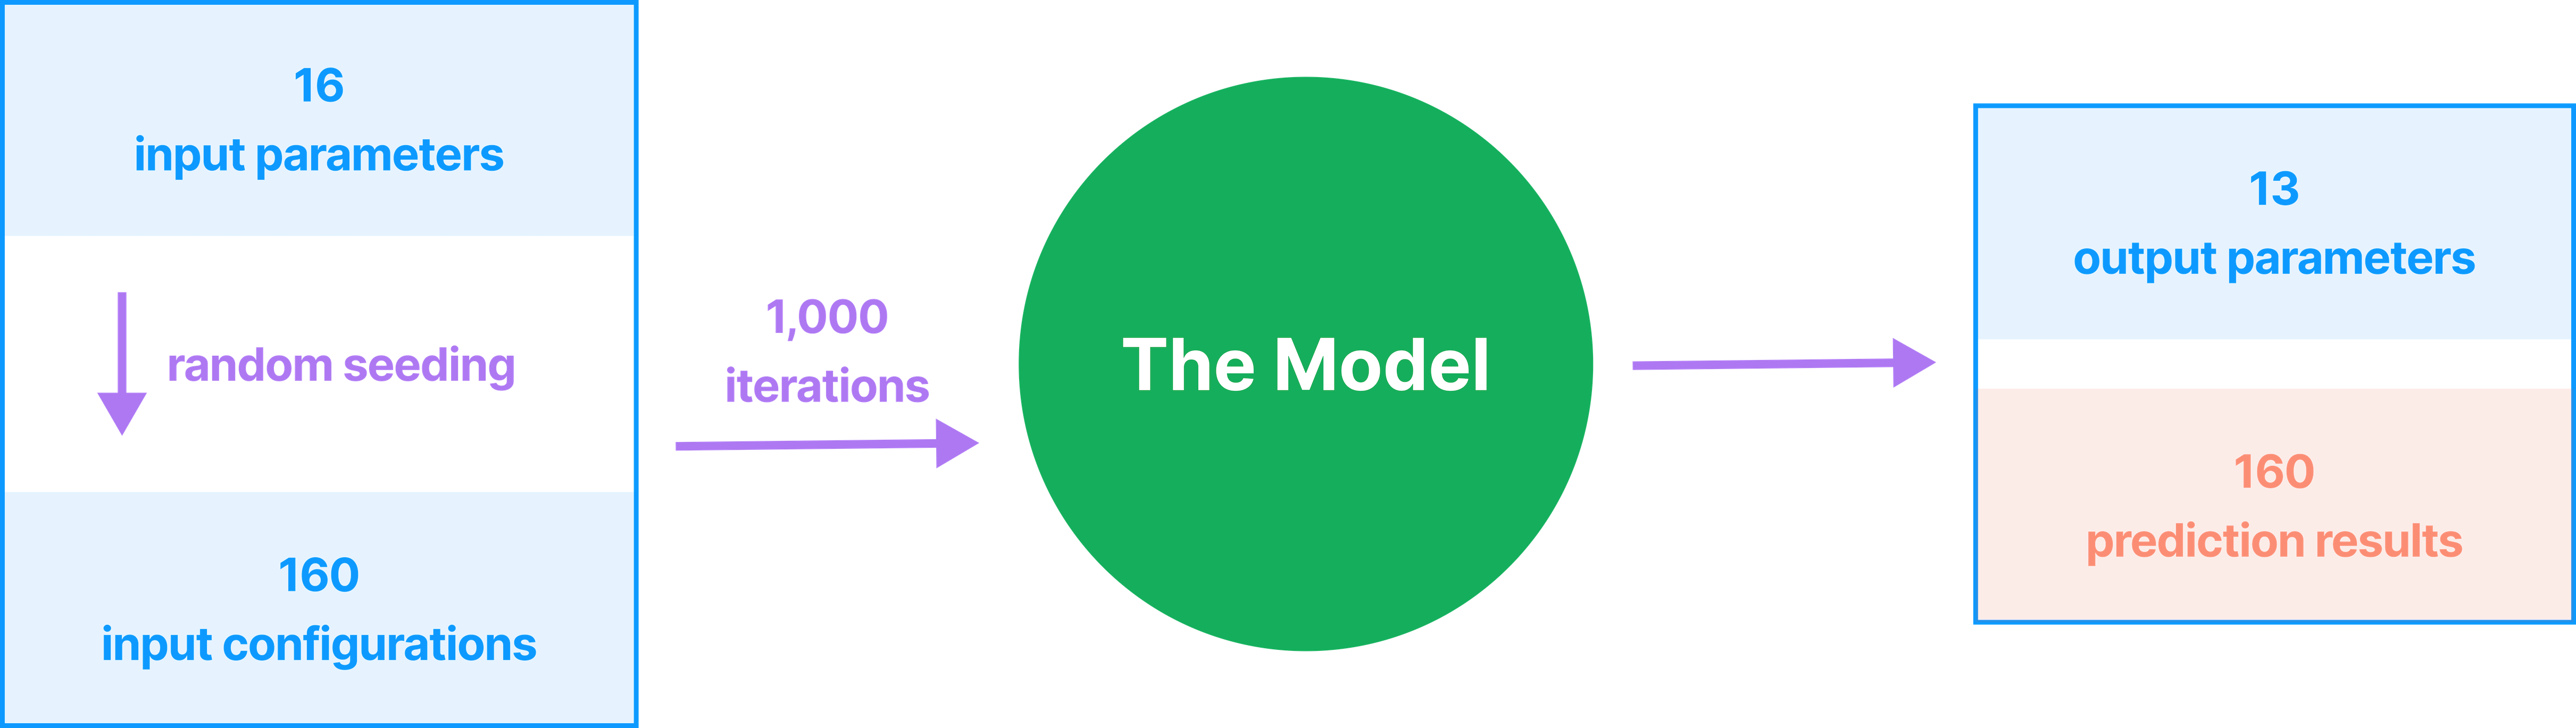
\includegraphics[width=\linewidth]{flow.png}
    \caption{An illustration of the flow from the input parameters to the prediction results. 160 sets of input parameters are used to perform 1,000 simulation iterations, resulting in 160 sets of prediction results.
    }
    \label{fig:flow}
\end{figure}

\end{samepage}



Upon receiving the data, we consulted the modelers to gain insights into the conventional workflow they employ for data processing, as well as the significance and the underlying meaning associated with each input and output parameter. As constant parameters such as $K$ and $rrd$ do not affect the simulation results, they are not rendered in our visual designs.

It is worth mentioning that after plotting the output data using a line chart, an error was immediately spotted, see \Cref{fig:1st-line}, where an unusual spike can be observed on day 20.
The modelers were notified and the bug was fixed.
However, the rectified output file was never made available to us.


\section{EnsembleVis}
\label{sec:EnsembleVis}

This section presents the experience behind our fully virtual collaboration between researchers from multiple UK institutions, chronicling the development of EnsembleVis.

% Change to paragraphs

\bobgraph{First Meeting - 27 July 2020}

\label{subsec:InitialMeeting}
On 27 July 2020, amid the UK's first national lockdown and stricter measures imposed by local authorities, we convened the initial virtual meeting with VIS researchers from King's College London, Loughborough University, Swansea University, University of Nottingham, University of Warwick, and University of Oxford.

During the meeting, we received an overview of the SCRC and the responsibilities of the visualization volunteer team.
Our assigned task was to create visualizations for the model, with the purpose of allowing the modelers to analyze the outcomes of the model.

Following the initial meeting, we engaged in email correspondence with the modelers to delve into the visualization requirements. The modelers shared a comprehensive list of parameters and model outcomes, along with the corresponding outcome data.

\bobgraph{First Commit - 14 Sep 2020}

We proceeded to create an initial prototype of the visualization, which was subsequently reviewed by the modelers.
Incorporating their input, we refined the prototype during our weekly internal discussions.
On 14 Sep 2020, England introduced the 'rule of six', which banned any gatherings above six.
On the same day, we made our first commit to a GitHub repository, signifying the commencement of our development.
At the same time, we began preprocessing the data.

A week after the initial commit, the UK witnessed the implementation of additional restrictions, such as mandatory work from home and a 10pm curfew.

\bobgraph{First Visualization, Second Meeting - 5 Nov 2020}

On 5 Nov 2020, the first day of the second national lockdown in the UK, we completed the first visualization, a parallel coordinates plot, see \Cref{fig:1st-vis}.
This followed by the second meeting with VIS researchers from other institutions, where we received feedback on the visualization, on 6 Nov 2020.

\begin{figure}[tb!]
    \centering
    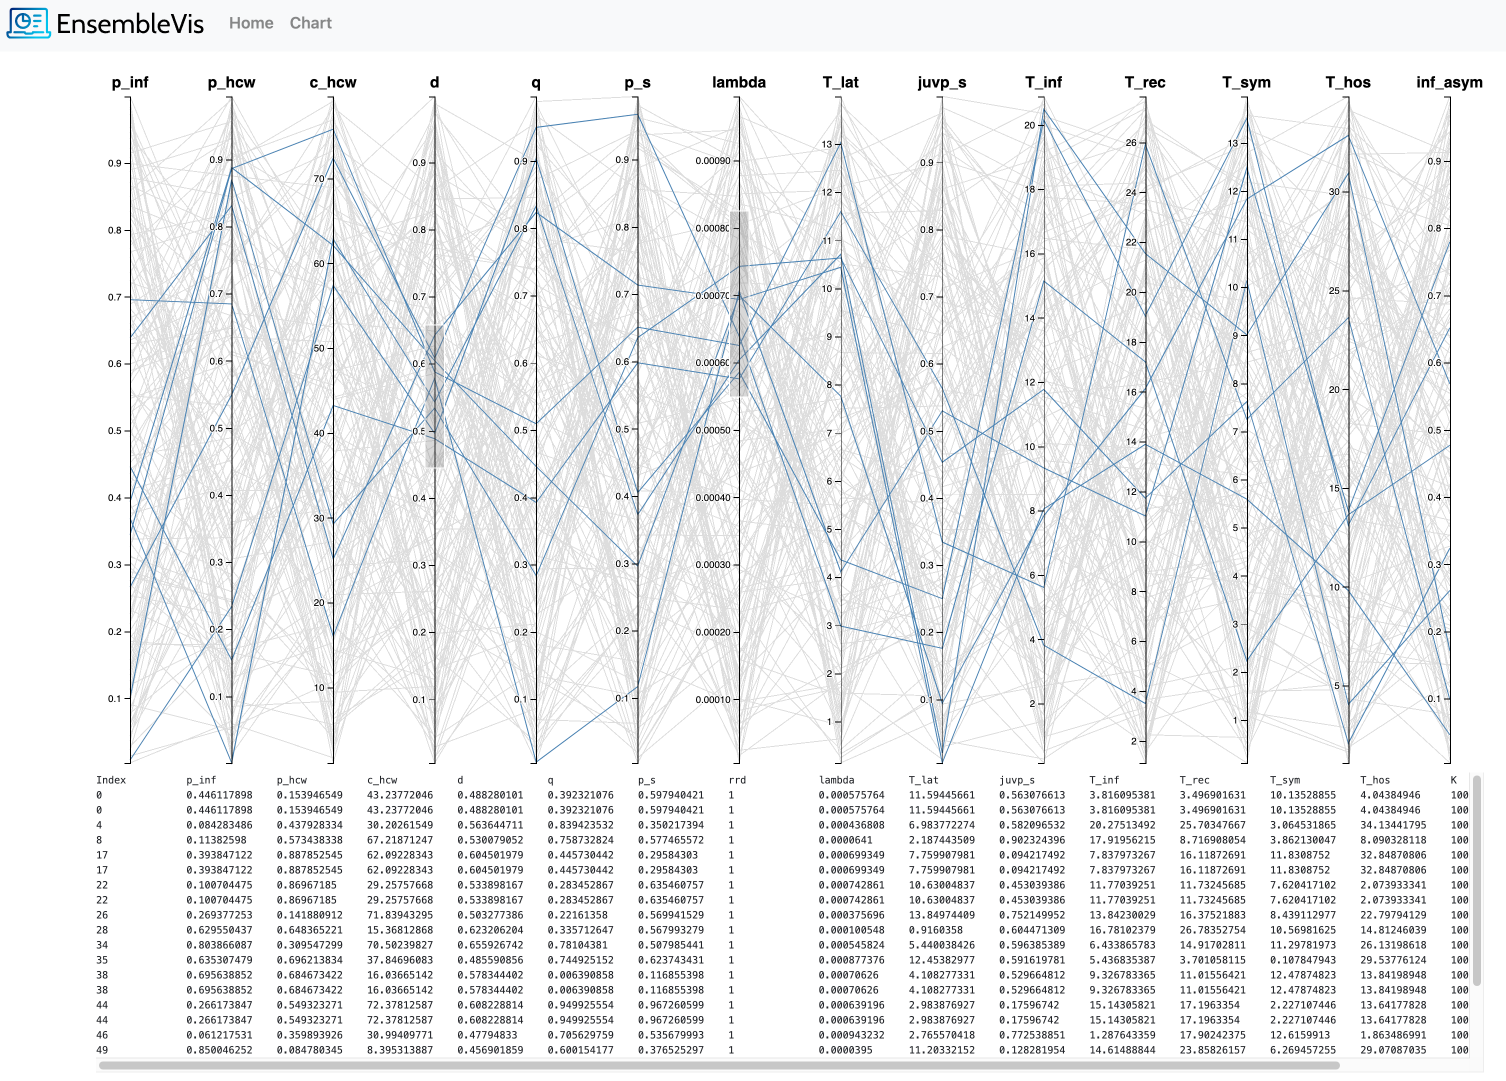
\includegraphics[width=\linewidth]{1st-vis.png}
    \caption{The first visualization, a parallel coordinates plot visualizing all 160 configurations of the model, was completed on 5 Nov 2020. This visualization was developed utilizing D3.js and incorporated a brushing feature, enabling users to filter the configurations.
    }
    \label{fig:1st-vis}

\end{figure}

\bobgraph{Third Meeting - 11 Nov 2020}

On 11 Nov 2020, the group convened for the third meeting, where we received further feedback on the visualization. As per the modelers' requests conveyed through emails, we incorporated a line chart to depict the model outcomes, see \Cref{fig:1st-line}.

\begin{figure}[tb!]
    \centering
    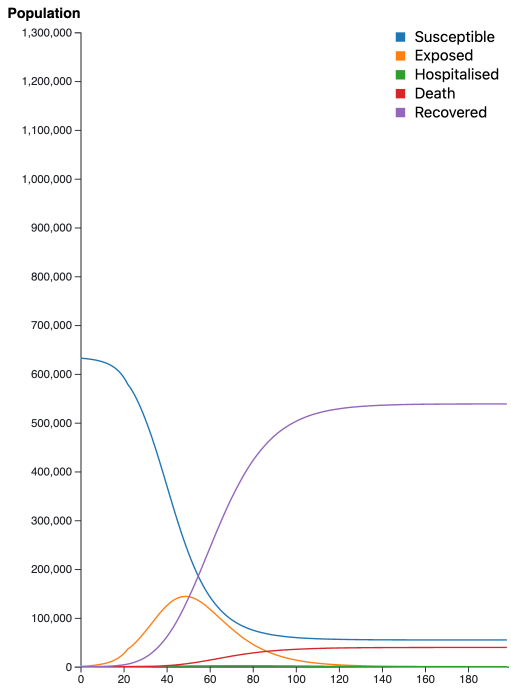
\includegraphics[width=\linewidth]{1st-line.png}
    \caption{A line chart was added to the visualization on 11 Nov 2020, to visualize the model outcomes.
    The x-axis of the chart corresponds to the number of days since the first available date in the Scottish dataset (specific date unknown to us), while the y-axis represents the population.
    To differentiate between different population categories, a color map was employed: susceptible (blue), exposed (orange), death (red), hospitalized (green), and recovered (purple).
    The final version of this chart which includes all the simulation results, is shown in \Cref{fig:teaser}D.
    }
    \label{fig:1st-line}

\end{figure}

\bobgraph{Fourth Meeting - 25 Nov 2020}

On 25 Nov 2020, the group convened for the fourth meeting, held just a day after the announcement of the gathering rules for Christmas in the UK.
During the meeting, we received feedback on the new visualization, a table with glyphs, see \Cref{fig:teaser}B. We incorporated this table view featuring glyphs to visualize all 160 input parameter configurations, following discussions with the modelers.
Each parameter is symbolized by a glyph, with the color of the glyph corresponding to its deviation from the average value.
The view provides the functionality to sort the parameters according to their values and can be dynamically updated by brushing the parallel coordinates plot for the input parameters (\Cref{fig:teaser}A).

\bobgraph{Fifth Meeting - 9 Dec 2020}

On 9 Dec 2020, a week after the end of the second national lockdown in the UK, with England facing a stricter three-tier restriction policy, the group convened for the fifth meeting.
At this point, we still had not met with the modelers, all communications and discussions took place through emails.

\bobgraph{Sixth Meeting - 10 Dec 2020}

On 10 Dec 2020, we finally met with modelers from the University of Edinburgh, the University of Exeter, the University of Glasgow, The London School of Hygiene \& Tropical Medicine, for the first time.
In contrast to sharing screenshots via email and deploying a website with a live view of our development (which they might not have been proficient in using), we delivered a live presentation, fielding numerous questions.
The modelers were extremely pleased with the visualization, and a list of feedback was provided:
\begin{enumerate}
    \item The modelers found the parallel coordinates plot very useful, and requested the incorporation of another one for the model outcomes. We implemented this as shown in \Cref{fig:teaser}C.
    \item The modelers requested all the simulation results to be displayed in \Cref{fig:1st-line}, with the current one being highlighted. We implemented this as shown in \Cref{fig:teaser}D.
    \item The modelers requested the incorporation of a scatterplot to visualize the model outcomes, specifically, a Principal Component Analysis (PCA) result obtained from other volunteers. We implemented this as shown in \Cref{fig:teaser}E.
\end{enumerate}

Furthermore, we received the exciting news that funding had been successfully secured, leading to the transition of our voluntary work to a team of paid developers, who would continue with further development of the project on a future date.

\bobgraph{Last Commit - 28 Apr 2021}

By 28 Apr 2021, the UK began a gradual easing of measures, although the prohibition on mixing between households was still in effect.
On this day, we made our last commit to the GitHub repository, this act signified the completion of our work, as we had smoothly transitioned all tasks to a team of paid developers.
The final version of our work is shown in \Cref{fig:teaser}.

During the entire development process, our meetings were exclusively conducted virtually, and our communication relied heavily on email correspondence.
Despite the lack of in-person interactions, we successfully met the modelers' requirements and delivered a highly satisfactory \ac{VIS} solution.


% \section{User-Centered Evaluation}


\section{Limitations}

Due to the impact of the pandemic, the project was conducted in a fully virtual manner, with all meetings and discussions taking place online, between a large group of researchers from different disciplines and different institutions.
\newtext{In total, 33 VIS researchers and 7 modelers were involved in this volunteer work.}
The development was ad-hoc in some ways due to the unprecedented nature of the pandemic.
This resulted in a number of limitations, which we will discuss in this section.

\subsection{Lack of Novel and Advanced Visual Designs}
Operating under a time constraint, the primary objective of our project centered on offering immediate visual analysis assistance to the modelers.
Thus, we were unable to explore the inclusion of innovative and advanced visual design approaches.
Instead, we integrated a series of classic views, such as line charts and scatterplots.
These are visual designs commonly leveraged by modelers and epidemiologists in their day-to-day research.
Interestingly, the modelers welcomed the introduction of a less conventional (to them) visualization technique: parallel coordinates.
They had never before employed this, and its introduction proved beneficial to their research.
Consequently, they expressed a desire for the incorporation of an additional parallel coordinates to assist in the visualization of model outcomes.

We believe that this is a testament to the effectiveness of advanced visual designs in enhancing the modelers' understanding of their models, this signals the possibility for future inclusion of more sophisticated visual designs.

\subsection{Lack of Proper Requirement Gathering}
We were unable to meet with the modelers and epidemiologists until the very last meeting. Instead, we had to rely on email correspondence, which was arguably not as effective as face-to-face or even virtual meetings.
In a traditional software engineering project, the requirements are gathered through a series of meetings and discussions with the end users. This did not occur in our case.

This resulted in a lack of proper requirement gathering, which in turn led to a number of challenges during the development process.
For example, the modelers made ad-hoc requests to incorporate different views at different stages of the project, resulting in unexpected changes on the development side.
This could have been avoided if we had a better understanding of their requirements from the beginning.

\subsection{Dynamic Group Membership}

The group membership was dynamic, with researchers joining and leaving the group at different stages of the project.
This introduced some lack of continuity, as newcomers had to spend time to familiarize themselves with the project.
Furthermore, members came from different disciplines, with different levels of expertise in visualization.
This has resulted in a lack of consistency in the development process, as different members have different ideas on how to implement the views.
The responsibility of each member, apart from the only developer in the group, was not clearly defined.

\subsection{Unclarified Project Direction}

The exact direction of the project was not clearly defined from the beginning.
Many details remained unknown to us during the development process, such as the exact purpose of the visualization, the target audience, and the end product. 
Consequently, the final product suffered from a non-ideal utilization of screen-space, as more views were requested to be added, the implementation of a multi-screen display design or collapsible views became time-constrained and unachievable.


\section{Conclusions}

In this paper, we present the stories behind the development of EnsembleVis, an interactive dashboard designed to visualize the input parameters and outcomes of an \ac{ABC-SMC} inference model used to analyze COVID-19 data collected during the first wave of the outbreak in Scotland.

Given the multitude of uncertainties and challenges during this exceptional period, a considerable amount of information was unavailable to us during the development process. It was only through the Scottish COVID-19 Response Consortium Stakeholder Report \cite{abdalla2021Scottish}, published in late 2021, and various publications \cite{chen2022RAMPVIS,dykes2022Visualizationb,khan2022Propagating,khan2022Rapid,rydow2023RAMPVIS} that unveiled the remarkable endeavors undertaken by other volunteer teams, that we gained additional insight and details.

\begin{figure}[tb!]
    \centering
    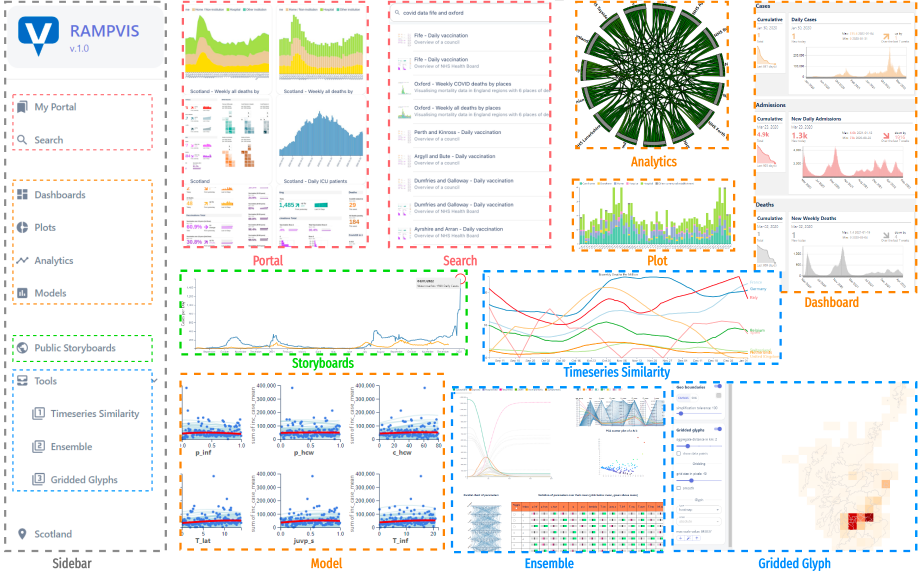
\includegraphics[width=\linewidth]{rampvis.png}
    \caption{EnsembleVis has undergone extensive development by multiple UK institutions and is currently maintained by the Oxford e-Research Centre at the University of Oxford, serving as a vital element of the RAMPVIS infrastructure. It is well-prepared to offer rapid and invaluable visualization support for future emergency responses. Image courtesy of Rydow et al. \cite{rydow2023RAMPVIS}.
    }
    \label{fig:rampvis}

\end{figure}

We hope that our experience serves as a valuable source of insight on how VIS research and techniques can play a crucial role in emergency response initiatives and aid in effectively preparing for future emergencies.

%% if specified like this the section will be committed in review mode
% \acknowledgments{
% The authors wish to thank A, B, and C. This work was supported in part by
% a grant from XYZ.}

%\bibliographystyle{abbrv}
% \bibliographystyle{abbrv-doi}
%\bibliographystyle{abbrv-doi-narrow}
\bibliographystyle{abbrv-doi-hyperref}
%\bibliographystyle{abbrv-doi-hyperref-narrow}

\bibliography{RAMPVIS}
\end{document}
